\documentclass[11pt]{scrartcl}
\usepackage[headheight=1pt, includeheadfoot, headsep=1cm, top=1.5cm, bottom=1.3cm, left=2cm, right=2cm]{geometry}
\usepackage{mathtools}
\usepackage{amsmath,amsthm, amscd, amssymb, amsfonts}
\usepackage[english]{babel}
\usepackage{fancyhdr}
\usepackage{enumitem}
\setlist{itemsep=0.5em}
\usepackage{xcolor}
\definecolor{forestgreen}{rgb}{0.13, 0.55, 0.13}
\usepackage[colorlinks = true,
linkcolor = forestgreen,
urlcolor  = forestgreen,
citecolor = forestgreen,
anchorcolor = forestgreen]{hyperref}
\usepackage{multicol}
\usepackage{multienum}
\usepackage{euler}
\usepackage[OT1]{eulervm}
\renewcommand{\rmdefault}{pplx}
\usepackage{tikz}
\usepackage{mathabx}
\usepackage{lastpage}



\usepackage{tikz}
\usepackage{verbatim}
\usetikzlibrary{shapes.geometric,shapes.multipart,arrows,calc}


\pgfdeclarelayer{background}
\pgfdeclarelayer{foreground}
\pgfsetlayers{background,main,foreground}			
\tikzset{
	edge/.style = {black, ultra thick, outer sep=2pt},
	vertex/.style = {draw=black, very thick, fill=white, circle, minimum width=8pt, inner sep=2pt, outer sep=1pt},
	arc/.style = {black, ultra thick, outer sep=2pt, decoration={markings, mark=at position #1 with {\arrow[scale=1.5]{latex}}}, postaction=decorate},
	arc/.default = 0.58
}


%% header, footer definitions
\def\course{MATH 314}
\def\courselink{https://www.gsanmarco.com/graph-theory}
\def\assignment{HW \#6}
\def\assignlink{hw06.tex}
\def\due{Due on Feb 28}




\pagestyle{fancy}
\fancyhead[L]{\course}
\fancyhead[C]{\assignment} 
\fancyhead[R]{\due} 
%\renewcommand{\footrulewidth}{0.4pt}
%\fancyfoot{}
%\fancyfoot[R]{\fontsize{8}{10} \selectfont  Page \thepage~of \pageref{LastPage}}
%\fancyfoot[L]{\fontsize{10}{12} \selectfont  Source file available at \href{\courselink}{\textbf{\courselink}}}

%% environments
% theorem style
\newtheorem{theorem}{Theorem}
\newtheorem{lemma}[theorem]{Lemma}
\newtheorem{corollary}[theorem]{Corollary}
\newtheorem{claim}[theorem]{Claim}
\newtheorem{defn}[theorem]{Definition}

% definition style
\theoremstyle{definition}
\newtheorem{problem}{Problem}
\newtheorem{Solution}{Solution}
% custom
\newenvironment{solution}{\noindent\textbf{Solution.}}{\qed}

%% custom commands

\newcommand*{\abs}[1]{\lvert #1\rvert}     % absolute values, cardinality
\newcommand*{\eps}{\varepsilon}            % prettier epsilon
\newcommand*{\R}{\mathbb{R}}               % real numbers
\newcommand*{\C}{\mathbb{C}}               % complex numbers
\newcommand*{\Q}{\mathbb{Q}}               % rational numbers
\newcommand*{\Z}{\mathbb{Z}}               % integers
\newcommand*{\N}{\mathbb{N}}               % natural numbers
\newcommand*{\F}{\mathbb{F}}               % field
\newcommand*{\family}{\mathcal{F}}         % family
\newcommand*{\GL}{\mathbf{GL}}             % general linear group
\newcommand*{\what}[1]{\widehat{#1}}       % wider hat
\newcommand*{\wbar}[1]{\overline{#1}}      % wider bar
\newcommand*{\mcal}[1]{\mathcal{#1}}       % mathcal
\newcommand*{\mbf}[1]{\mathbf{#1}}         % mathbf
\newcommand*{\mbb}[1]{\mathbb{#1}}         % mathbb

% operators
\let\Pr\relax\DeclareMathOperator*{\Pr}{\mathbf{Pr}}       % probability
\DeclareMathOperator*{\E}{\mathbb{E}}          % expectation
\DeclareMathOperator*{\Var}{\mathbf{Var}}      % variance
\DeclareMathOperator*{\Span}{span}             % span
\DeclareMathOperator{\tr}{tr}                  % trace
\DeclareMathOperator{\rank}{rank}              % rank
\DeclareMathOperator{\supp}{supp}              % support
\DeclareMathOperator{\diam}{diam}



\begin{document}
\noindent  Unless explicitly requested by a problem, do not include sketches as part of your proof. You are free to use the result from any problem on this (or previous) assignment as a part of your solution to a different problem even if you have not solved the former problem.
\vskip10pt

\begin{problem}[0.5 + 0.5 pts]
	Determine the Pr\"ufer code of the following trees, using the ordering $v_1\leq v_2\leq \dots$ for the vertices.
\begin{multicols}{2}
\begin{enumerate}[leftmargin=*, label=(\alph*)]
	\item \phantom{hi}
	\begin{center}
		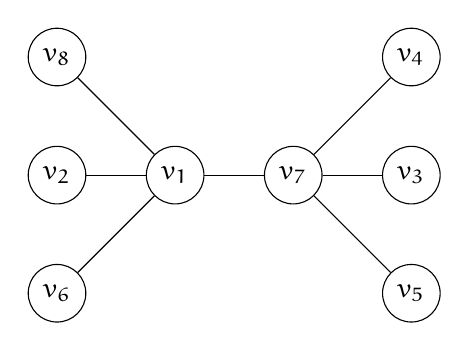
\begin{tikzpicture}[main/.style = {draw, circle}, scale = 1.5]
			\node[main] (1) at (0,0) {$v_1$};
			\node[main] (2) at (-1,0) {$v_2$};
			\node[main] (3) at (2,0) {$v_3$};
			\node[main] (4) at (2,1) {$v_4$};
			\node[main] (5) at (2,-1) {$v_5$};
			\node[main] (6) at (-1,-1) {$v_6$};
			\node[main] (7) at (1,0) {$v_7$};
			\node[main] (8) at (-1,1) {$v_8$};
			\draw (2)--(1)--(7)--(3);
			\draw (8)--(1)--(6);
			\draw (4)--(7)--(5);
		\end{tikzpicture}
	\end{center}
	\item \phantom{hi}
	\begin{center}
		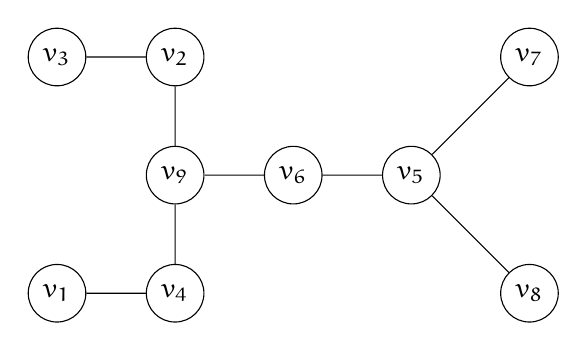
\begin{tikzpicture}[main/.style = {draw, circle}, scale = 1.5]
			\node[main] (1) at (1,-1) {$v_1$};
			\node[main] (2) at (2,1) {$v_2$};
			\node[main] (3) at (1,1) {$v_3$};
			\node[main] (4) at (2,-1) {$v_4$};
			\node[main] (5) at (4,0) {$v_5$};
			\node[main] (6) at (3,0) {$v_6$};
			\node[main] (7) at (5,1) {$v_7$};
			\node[main] (8) at (5,-1) {$v_8$};
			\node[main] (9) at (2,0) {$v_9$};
			\draw (1)--(4)--(9)--(6)--(5)--(8);
			\draw (3)--(2)--(9);
			\draw (7)--(5);
		\end{tikzpicture}
	\end{center}
\end{enumerate}
\end{multicols}
\end{problem}
\begin{solution}
\begin{enumerate}[leftmargin=*, label=(\alph*)]
	\item $(1,7,7,7,1,1)$
	\item $(4,2,9,9,5,5,6)$
\end{enumerate} 
\end{solution}

\hrulefill

\begin{problem}[0.5 + 0.5 pts]
	For the following sequences, draw a picture of the (labeled) tree which has that sequence as its Pr\"ufer code (using the standard ordering of the integers).
	Your tree should have vertex-set $\{v_1, \dots, v_n\}$ for some integer $n$.
\begin{multicols}{2}
	\begin{enumerate}[leftmargin=*, label=(\alph*)]
		\item $(v_5,v_7,v_5,v_1,v_3,v_5,v_5)$
		\item $(v_4,v_4,v_1,v_2,v_1,v_2,v_3)$
	\end{enumerate}
\end{multicols}
\end{problem}

\begin{solution}
\begin{enumerate}[leftmargin=*, label=(\alph*)]
	\item \phantom{hi}
	\begin{center}
		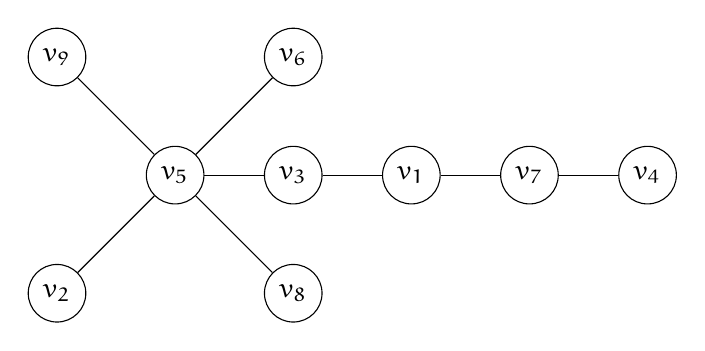
\begin{tikzpicture}[main/.style = {draw, circle}, scale = 1.5]
			\node[main] (1) at (0,0) {$v_1$};
			\node[main] (2) at (-3,-1) {$v_2$};
			\node[main] (3) at (-1,0) {$v_3$};
			\node[main] (4) at (2,0) {$v_4$};
			\node[main] (5) at (-2,0) {$v_5$};
			\node[main] (6) at (-1,1) {$v_6$};
			\node[main] (7) at (1,0) {$v_7$};
			\node[main] (8) at (-1,-1) {$v_8$};
			\node[main] (9) at (-3,1) {$v_9$};
			\draw (5)--(3)--(1)--(7)--(4);
			\draw (9)--(5)--(2);
			\draw (6)--(5)--(8);
		\end{tikzpicture}
	\end{center}
	\item \phantom{hi}
\begin{center}
	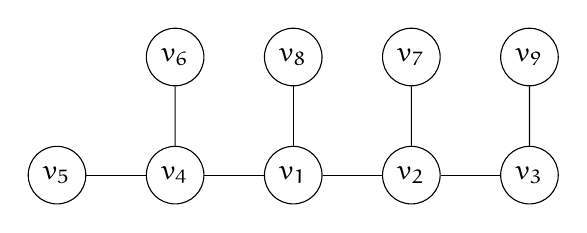
\begin{tikzpicture}[main/.style = {draw, circle}, scale = 1.5]
		\node[main] (1) at (0,0) {$v_1$};
		\node[main] (2) at (1,0) {$v_2$};
		\node[main] (3) at (2,0) {$v_3$};
		\node[main] (4) at (-1,0) {$v_4$};
		\node[main] (5) at (-2,0) {$v_5$};
		\node[main] (6) at (-1,1) {$v_6$};
		\node[main] (7) at (1,1) {$v_7$};
		\node[main] (8) at (0,1) {$v_8$};
		\node[main] (9) at (2,1) {$v_9$};
		\draw (5)--(4)--(1)--(2)--(3);
		\draw (6)--(4);
		\draw (8)--(1);
		\draw (7)--(2);
		\draw (9)--(3);
	\end{tikzpicture}
\end{center}
\end{enumerate}
\end{solution}

\hrulefill

\begin{problem}[1 pts]
	Determine (with proof) all trees $T$ (up to isomorphism) on $n\geq 2$ vertices whose Pr\"ufer code uses each element of $V(T)$ at most once (under any arbitrary ordering of $V(T)$).
\end{problem}

\begin{solution}
Under any ordering of $V(T)$, we saw in class that the symbol $x\in V(T)$ appears exactly $\deg_Tx -1$ many times in the Pr\"ufer code of $T$. Therefore, $x$ appears at most once in the Pr\"ufer code of $T$ if and only if $\deg_T x \leq 2$. In other words, the Pr\"ufer code of $T$ sees each element of $V(T)$ at most once if and only if $\Delta(T)\leq 2$. This happens if and only if $T\cong P_n$ as per HW4.3.
\end{solution}

\hrulefill

\begin{problem}[2 pts]
	Fix an integer $n\geq 2$ and let $d_1,\dots,d_n$ be a sequence of positive integers with $\sum_{i=1}^nd_i=2n-2$.
	Use Pr\"ufer codes to show that there is a tree with degree sequence $d_1,\dots,d_n$.
\end{problem}

\begin{solution}
Fix a vertex-set $V=\{v_1, \dots, v_n\}$ with an arbitrary order, say $v_1<v_2<\dots<v_n$. Let $\mathcal T_V$ denote the family of all trees on this vertex-set. 

Consider the following tuple of elements in $V$:
\[P=( \underbrace{v_1, \dots, v_1}_{d_1 -1 \text{times}}, \underbrace{v_2, \dots, v_2}_{d_2 -1 \text{times}}, \dots,  \underbrace{v_n, \dots, v_n}_{d_n -1 \text{times}})\]
Observe that this makes sense because each $d_i-1$ is a non-negative integer. Moreover, the number of entries in $P$ is 
\[ \sum_{i=1}^{n}(d_i -1 ) = \sum_{i=1}^{n}d_i  - n = 2n-2- n= n-2 \]
Thus $P \in V^{n-2}$. Since $\textrm{Pr\"ufer}_V \colon \mathcal T_V \to V^{n-2}$ is a bijection, there is a (unique) tree $T\in \mathcal T_V$ such that $\textrm{Pr\"ufer}_V (T)=P$. We saw in class that $\textrm{Pr\"ufer}_V (T)$ contains each vertex $v_i$ exactly $\deg_T v_i -1$ times. Thus $\deg_T v_i -1= d_i-1$, or in other words $\deg_T v_i = d_i$ for all $i\in \{1,\dots, n\}$. Thus the degree sequence of $T$ is $d_1,\dots,d_n$.
\end{solution}

\hrulefill

\begin{problem}[2 pts]
	For a graph $G$, define the relation $R$ on $V(G)$ by $u\mathbin R v$ if and only if $u=v$ or there is a cycle in $G$ containing both $u$ and $v$.
	Find a graph $G$ wherein $R$ is \emph{not} an equivalence relation on $V(G)$.
	(You are welcome to define $G$ via a picture, though, of course, you must still demonstrate that $R$ is not an equivalence relation on this $G$)
\end{problem}

\begin{solution}
Consider the following graph
\begin{center}
	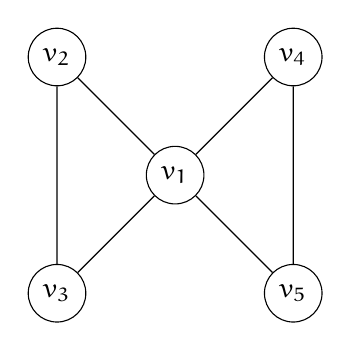
\begin{tikzpicture}[main/.style = {draw, circle}, scale = 1.5]
		\node[main] (1) at (0,0) {$v_1$};
		\node[main] (2) at (-1,1) {$v_2$};
		\node[main] (3) at (-1,-1) {$v_3$};
		\node[main] (4) at (1,1) {$v_4$};
		\node[main] (5) at (1,-1) {$v_5$};
		\draw (1)--(2);
		\draw (1)--(3);
		\draw (2)--(3);
		\draw (1)--(4);
		\draw (1)--(5);
		\draw (4)--(5);
	\end{tikzpicture}
\end{center}
Observe that $v_2\mathbin R v_1$, as witnessed by the cycle $(v_1, v_2, v_3)$. Similarly, $v_1\mathbin R v_4$, as witnessed by the cycle $(v_1, v_4, v_5)$. However, there is no cycle containing $v_2$ and $v_4$, thus $v_2$ is not related to $v_4$. Hence $R$ is not transitive, so it is not an equivalence relation.
\end{solution}

\hrulefill
\begin{problem}[3 pts]
	For a graph $G$, define the relation $R$ on $E(G)$ by $e\mathbin R s$ if and only if $e=s$ or there is a cycle in $G$ containing both $e$ and $s$.
	Prove that $R$ is an equivalence relation on $E(G)$.
\end{problem}

\begin{solution}
Reflexivity is obvious since $e = e$ for any edge $e\in E(G)$. Symmetry is also obvious since if there is a cycle containing both $e$ and $s$, then this same cycle contains both $s$ and $e$.

Transitivity is the only interesting part. Suppose that $e\mathbin R s$ and $s\mathbin R t$; we must show that $e\mathbin R t$. If either $e = s$ or $s = t$, then this is immediate, so we may suppose that $e$, $s$, $t$ are three distinct edges. 

Thus, let $C_{es}$ be a cycle in $G$ containing both $e$ and $s$, and let $C_{st}$ be a cycle in $G$ containing both $s$ and $t$. Label $C_{es} = (v_1,\dots, v_k)$ where $e = v_1v_k$ and label $C_{st} = (u_1,\dots, u_\ell)$ where $t = u_1u_\ell$; of course, $k,\ell\geq3$. Let $i$ be the smallest index for which $v_i \in \{u_1,\dots,u_\ell\}$ and let $j$ be the largest index for which $v_j\in \{u_1,\dots, u_\ell\}$; we begin by showing that both $i, j$ exist and that $i< j$. Indeed, $s$ belongs to both $C_{es}$ and to $C_{st}$ and so $s=v_av_{a+1}$ and $s=u_bu_{b+1}$  for some $a\in \{1, \dots, k-1\}$ and some $b\in \{1, \dots, \ell -1\}$ (since $e\ne s$ and $t\ne s$).  In particular, $v_a,v_{a+1} \in\{u_1,\dots, u_\ell\}$ and so $1\leq i\leq a< a+1\leq j\leq k$. Suppose that $v_i = u_{i'}$ and $v_j = u_{j'}$ for some $i', j' \in \{1,\dots, \ell\}$; of course $i'\neq j'$. By the definition of $i$ and $j$, we know that $\{v_1,\dots, v_{i-1}\} \cap  \{u_1, \dots , u_\ell\} = \{v_k,\dots , v_{j+1}\} \cap \{u_1,\dots, u_\ell\} = \emptyset$.

If $i' <j'$, consider the sequence $C=(v_1,\dots,v_i =u_{i'},u_{i'-1}\dots,u_1,u_\ell,u_{\ell-1},\dots,u_{j'} =v_j,v_{j+1},\dots ,v_k)$,  and if $i'>j'$, consider the sequence $C =(v_1,\dots ,v_i =u_{i'},u_{i'+1},\dots ,u_\ell,u_1,u_2,\dots, u_{j'} =v_j,v_{j+1},\dots,v_k)$. By the earlier remark, in either case, $C$ forms a cycle. Furthermore, since $e = v_1v_k$ and $t = u_1u_\ell$, we see that $C$ forms a cycle in $G$ containing both $e$ and $t$; thus $e \mathbin R t$ as needed.
\end{solution}
\end{document}




